\section{Dampak Konvensi Panggilan (Calling Conventions)}

Alokasi register tidak terjadi dalam ruang hampa; ia harus mematuhi aturan interaksi antar fungsi yang didefinisikan oleh \compiler{Application Binary Interface (ABI)}.

\subsection{Caller-Saved vs Callee-Saved}
ABI membagi register menjadi dua kategori utama yang memaksa kompilator melakukan penghematan (\textit{saving}) secara strategis:
\begin{enumerate}
    \item \textbf{Caller-Saved} (Volatile): Register yang nilainya boleh dirusak oleh fungsi yang dipanggil. Jika pemanggil (\textit{caller}) masih membutuhkan data tersebut setelah panggilan fungsi, ia harus menyimpannya ke \textit{stack} sebelumnya.
    \item \textbf{Callee-Saved} (Non-volatile): Register yang nilainya harus dijaga. Jika fungsi yang dipanggil (\textit{callee}) ingin menggunakannya, ia wajib menyimpan nilai aslinya di awal fungsi dan mengembalikannya sebelum selesai.
\end{enumerate}

\subsection{Strategi Penempatan Variabel}
Kompilator yang cerdas menggunakan informasi ini untuk optimasi:
\begin{itemize}
    \item \textbf{Variabel Berumur Panjang} (melewati banyak panggilan fungsi): Sebaiknya diletakkan di \textbf{Callee-Saved registers}. Ini menghindari biaya \textit{save/restore} di setiap titik pemanggilan fungsi.
    \item \textbf{Variabel Berumur Pendek} (tidak melewati panggilan fungsi): Sebaiknya diletakkan di \textbf{Caller-Saved registers} karena tidak ada risiko data tersebut dihancurkan oleh fungsi lain.
\end{itemize}

\begin{figure}[!htbp]
    \centering
    \adjustbox{max width=0.8\textwidth,center}{%
    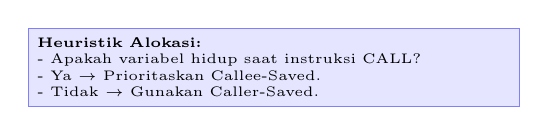
\begin{tikzpicture}[
        rect/.style={rectangle, draw=blue!50, fill=blue!10, text width=6cm, font=\tiny}
    ]
    \node[rect] (strat) {
        \textbf{Heuristik Alokasi:}\\
        - Apakah variabel hidup saat instruksi CALL?\\
        - Ya $\rightarrow$ Prioritaskan Callee-Saved.\\
        - Tidak $\rightarrow$ Gunakan Caller-Saved.
    };
    \end{tikzpicture}%
    }
    \caption{Strategi Pemilihan Register Berbasis Konvensi Panggilan}
\end{figure}
